% !TEX root = ../Dissertation.tex
%===================================================================================================

\chapter{Introduction}


\section{Diabetes - Facts and Figures}
\label{sec:sectionLabel}


Diabetes mellitus is a condition affecting the body's ability to control blood sugar levels.
According to statistics provided by Diabetes UK, diabetes affects approximately 3.9 million people in the UK, with many more sufferers, as yet, undiagnosed.
The incidence of diabetes is rising rapidly, with the prevalence of diabetes in the UK now being more than double that of 1996 \citep{DiabetesUK}.


Diabetes results from either lack of, or resistance to, the hormone insulin.
The pathogenesis of the disease depends on the type of diabetes in question.
There are a few types of diabetes including gestational diabetes, seen in some pregnancies, type 1 diabetes, and type 2 diabetes.
Type 1 diabetes (T1D) is an autoimmune condition where the body's own immune system destroys insulin producing cells, resulting in a lack of insulin.
Type 2 diabetes (T2D), on the other hand, is when the body becomes resistant to the action of insulin and insulin production is impaired.
Both type 1 and type 2 diabetes result in a decreased ability to regulate blood glucose levels.

Insulin is produced in the pancreas by $\beta$ cells in the Islets of Langerhans.
It is a vitally important hormone involved with the maintenance of normal blood glucose levels, in particular stopping dangerous rises in blood glucose levels.
Insulin's main actions are to stop the production of extra glucose when blood glucose is already sufficiently high.
It does this by keeping the brakes on mechanisms of glucose production such as glycogenolysis (breakdown of glycogen stores), lipolysis (breakdown of fats) and proteolysis (breakdown of protein).
It also prevents the production of glucagon, the hormone which acts to raise glucose levels \citep{Sonksen2000}.

The dysregulation of blood glucose levels seen in diabetes is what causes the many complications seen in the disease.
It is, therefore, crucial for the patient to carefully monitor and control blood glucose either by diet or medication, depending on type and severity of the diabetes.
Alongisde the charactistic diabetes symptoms of excessive thrist, drinking and urination, there are serious side effects both in the short and longer term.
In the short term, extremes of blood glucose, either too high or too low can lead to hyper- or hypoglycaemia which require fast treatment in order to prevent potentially lethal conditions such as diabetic ketoacidosis in T1D, or hyperosmolar hyperglcaemic state in T2D.
In the longer term, prolonged mild hyperglycaemia caused by diabetes can cause micro- and macrovascular complications leading to blindness, neuropathy, kidney failure and a significantly increased risk of cardiovascular disease\citep{OxClinMed}.
It is therefore vitally important for research into diabetes to continue, with the aim of finding a cure.

\subsection{Type 1 Diabetes}

This project is concerned only with type 1 diabetes (T1D).
T1D is a serious autoimmune condition whereby the host's own immune system destroys $\beta$ cells in the pancreatic Islets of Langerhans.
Destruction of $\beta$ cells results in a lack of insulin and forces the patient to rely on self monitoring of blood glucose through regular finger prick blood testing and subsequent insulin administration.
Until recently it was thought that T1D led to a total obliteration of $\beta$ cells, however, it is now thought that very small numbers of $\beta$ cells remain and are able to secrete insulin \citep{Oram2014, Veld2014}.
Type 1 diabetes affects approximately 10\% of all diabetes sufferers \citep{DiabetesUK}.




%However, in T1D, the resulting lack of insulin means that these processes cannot be kept in check causing subsequent hyperglycaemia \citep{Sonksen2000}.
%The total lack of insulin production ability in T1D means that effective glucose monitoring and self administration of glucose via injection or infusion is cruicial to maintain blood glucose homeostasis.

%There are two kinds of diabetes mellitus, type 1 and type 2.
%Type 1 Diabetes (T1D) is a serious autoimmune condition whereby the body's own immune system destroys the insulin producing beta cells in the pancreatic Islets of Langerhans \citep{Daneman2006}.
%Type 2 Diabetes, however, is a condition where the body becomes either resistant to insulin or the insulin producing beta cells become dysfunctional.
%Whereas T1D is an antoimmune disease with typical onset during adolescence, T2D is more prevalent in older people and is linked to changes in lifestyle \citep{OxClinMed}.
%This project is concerned with T1D and it's autoimmune basis.

%According to statistics provided by Diabetes UK, diabetes, both T1D and T2D, affects approximately 3.9 million people in the UK, with many more as yet undiagnosed. 
%Of all diabetes sufferers, around 10\% have T1D \toref{Diabetes UK 2015}.





%There are currently two arms of T1D research.
%The first involves using diabetic patients.
%This has it's limitations due to the lack of tissue availability and because a lot of the beta cell destruction occurs prior to the appearance of T1D symptoms \citep{Thomas2000}.
%The other arm requires the use of animal models, particularly the nonobese diabetic (NOD) mouse, which is currently the best available animal model of T1D.
%The NOD mouse will be discussed further below.

\section{The Immune system}
\subsection{Role}

The immune system evolved to protect animals from a variety of pathology-inducing agents such as bacteria, protozoa, viruses and fungi.
The immune system is designed to recognise invading pathogens and eliminate them before they can cause harm to the host.
The immune system consists of two interconnecting arms known as the innate immune system and the adaptive immune system.
The innate system is the more primitive, non specific system whereas the adaptive immune system is highly specific and capable of recognising unique components on pathogens in order to mount the best possible response towards it.
The cells and processes involved in each arm of the immune system are different but are interconnected through cell-cell interactions and cytokine and chemokine secretion. \todo{Add some references}

\subsection{Innate}

The innate immune system is characterised by being non specific, fast acting and incapable of forming immunological memory.
The aim of the system is to prevent entry of pathogens and recognise, engulf and destroy pathogens which have managed to invade.
Following this, pathogenic antigens are presented to cells of the adaptive immune system and inflammatory cytokines are produced to signal to other immune cells and boost the immune response.

The innate immune system has numerous ways of preventing pathogen entry, such as the skin and epithelial tight junctions providing physical barriers and enzymes, antimicrobial peptides and mucus to catch and kill pathogens trying to enter.

However, should microorganisms gain entry to the body, there are innate immune cells which can take over.
These include phagocytes (macrophages, dendritic cells (DCs) and neutrophils) and natural killer (NK) cells. 
To recognise invading pathogens, cells of the innate immune system have a number of different receptors, both membrane bound and free in the cytosol.
These pattern recognition receptors (PRRs), such as Toll-like receptors (TLRs), C-type Lectins, NACHT-leucine rich repeat receptors (NLRs) and Rig-like receptors (RLRs) are capable of recognising a variety of patterns expressed only by microbes, known as pathogen-associated molecular patterns (PAMPs).
Binding through receptors such as these transmits signals into the cells resulting in subsequent release of inflammatory cytokines, upregulation of major histocompatibility complex (MHC) Class II, upregulation of costimulatory molecules (vital for antigen presentation, see below), and upregulation of killing mechanisms following phagocytosis of pathogens.
The ability to recognise these PAMPs gives the innate immune system to ability to distinguish self from non-self.

However, the immune system is not only there to protect from invading organisms. 
Damaged host cells also require removal by the immune system  to prevent inflammation and potential autoreactive responses. 
In order to do this, it is thought that the innate immune system is also able to recognise damage-associated molecular patterns (DAMPs) which can also bind to TLRs and ellicit an immune response \citep{Matzinger1994, Shin2015}

\todo{Add some references}

\subsection{Adaptive}

The adaptive immune system is different from the innate immune system in that it is slower acting, highly specific and has the ability to form immunological memory.
The adaptive immune system is concerned with tailoring the immune response to a specific pathogen.

The adaptive immune system is composed of T and B lymphocytes, also known as T and B cells.
These cells express receptors which are specific to a given antigen.
Each T and B cell has a different antigen specificity therefore the adaptive immune system can recognise a huge number of antigens via B and T cell receptors.

However, B and T cells require activation before they can function.
In order to activate these cells, they must first encounter their cognate antigen (i.e, the antigen for which their receptor is specific).
B cells are capable of recognising whole protein, whereas T cells require their antigen to be degraded into peptide fragments and presented to them by antigen presenting cells.
%Activation results in proliferation of the clone able to recognise the antigen and therefore, a highly specific army of effector cells capable of fighting the pathogen is formed.
%The process of antigen presentation and T cell activation will be described more fully in \cref{subsec:Tcellactivation}.
Once activated, B and T cells are able to carry out their functions.

The functions of the adaptive immune cells vary.
T cells have many different subsets with differing functions depending on the subset.
Some are concerned with orchestrating the overall immune response (T helper cells) while others are designed to kill their target cells directly (killer T cells).
These will be discussed in more detail in \cref{subsec:Tcellfunctions}.
B cells, on the other hand, are capable of antigen presentation but their main function is antibody production.
Antibodies are the secreted form of the B cell receptor and are designed to help with removal of the pathogen by phagocytosis or complement (a process consisting of a variety of different proteins aimed at the destruction of pathogens) and to help neutralise harmful toxins produced by microorganisms.

\subsection{Receptor Rearrangement}
\label{subsec:receptorrearrangement}

T and B cells both have receptors known as TcR and BcR respectively.
Each B and T cell has a unique receptor which results in a massive repertoire (approximately 10\textsuperscript{13-14} possible receptors \citep{KubyImmunology}) of B and T cell receptors, each capable of responding to a different antigen.
Due to both types of receptor requiring a huge potential for diversity, the mechanisms which introduce this diversity are largely the same for both receptor types.


There are two types of TcR, each consisting of two chains.
The main one is an $\alpha\beta$ receptor which is most common, and the second is a $\gamma\delta$ receptor.
In the BcR, there are also two chains, known as the heavy and light chain.
The heavy chain is equivalent to either the $\beta$ or $\delta$ chains, while the light chain is equivalent to the $\alpha$ or $\gamma$ chains.

The receptor chains consist of a variable and constant region.
The variable region is the part which is capable of recognising antigen, whilst in BcRs, the constant region gives the immunoglobulin it's class.

The variable region is made up of V (variable), D (diversity, heavy, $\beta$ and $\delta$ chains only) and J gene segments.
Genomically encoded are multiple copies of different V, D and J genes and during rearrangement, one of each of these genes are selected at random and joined to produce different receptors.
This process is mediated by enzymes known as RAG (recombination activating genes) recombinases.
These enzymes recognise recombination signal sequences (RSS) found next to the coding regions of each V, D and J gene and bring the ends of the chosen genes near to each other to be joined \citep{Fugmann2014, Oettinger1999}.
To join the segments, RAG proteins cleave at either end of the genes and leave hairpin loops of DNA.
From here a nuclease nicks the loops leaving short sequences at the end of each gene to be joined.
This allows the segments to join via non homologous end joining \citep{Schatz2011}.
Further diversity is also added via the use of an enzyme called terminal deoxynucleotidyltransferase (TdT) which adds random base pairs between each segment.
%The use of TdT allows the production of the ~10\textsuperscript{14} different immunoglobulins \citep{Motea2010}.

TcRs are able to respond to their antigen peptides held in major histocompatibility complexes (MHC) on APCs, whereas BcRs are able to respond to whole antigens.

%\subsection{Antigen presentation}

%For T cells to be able to recognise their antigen, APCs must present the antigen to them in petide form, held in MHC on the APC's surface.

%\todo{MHC presentation pathways - MHC Class II and MHC Class I. Presentation only, T cell activation covered later}


\section{T cells}



\subsection{Development}
\label{subsec:Tcelldevelopment}

T cells develop in the thymus.
Since the thymus does not contain self-renewing thymocytes, the process of T cell development relies on the constant seeding of the thymus by progenitors from the bone marrow \citep{Zlotoff2011, Heinzel2007}.
However, the cell that is responsible for this seeding and acts as a T cell progenitor is not known.
There are many candidates and these have been identified by looking at the surface markers that are required for a cell to be able to settle in the thymus and develop into a T cell.

Haematopoietic stem cells (HSCs) are the progenitors from which all blood cells derive.
These cells are found in the bone marrow and, via the production of various progenitors, can produce megakaryocytes, erythrocytes, lymphocytes, granulocytes, macrophages and natural killer cells.
HSCs are characterised by their lineage (lin)\textsuperscript{-} stem cells antigen-1 (Sca-1)\textsuperscript{high} stem cell growth factor receptor (c-kit)\textsuperscript{high} expression (so-called LSK cells) and lack of surface fms-like tyrosine kinase 3 (Flt3) \citep{Welinder2011}.

Following the HSC stage, multipotent progenitors (MPPs) form which have the capability of producing all types of blood cell, but lack the self-renewing ability of HSCs.
These cells are LSK but also express Flt3\textsuperscript{low} \citep{Welinder2011}.
Interestingly, MPPs can express genes of multiple lineages \citep{Hu1997} suggesting that this expression is due to priming for lineage committment, rather than commitment itself.
It is thought that by expressing these genes, it maintains them in an accessible chromatin state, ready for commitment \citep{Welinder2011}.
Evidence for this has been seen through changes in chromatin staus of lineage restricted genes during blood cell development \citep{Weishaupt2010}.

Following MPP development, magakaryocytic and erythrocytic potential is much reduced and the so-called lymphoid primed multipotent progenitor (LMPP) arises.
These cells are capable only of lymphocyte, macrophage, granulocyte and NK cell production \citep{Adolfsson2005}.
LMPPs are characterised by being LSK but also Flt3\textsuperscript{high}.

Next, the interleukin-7 receptor-$\alpha$ (Il-7R$\alpha$) upregulates and Sca-1 and c-kit downregulate to form common lymphoid progenitors (CLP).
These cells are capable only of B and T lymphocyte development and NK cell development \citep{Kondo1997} and are Sca-1\textsuperscript{low} c-kit\textsuperscript{low} Flt3\textsuperscript{+} Il-7R$\alpha$\textsuperscript{+}.
Flt3 is the receptor for Flt3 ligand (Flt3L) which is found in the bone marrow and acts as a growth promoter for CLPs.
Flt3L also works synergistically with IL-7 to promote lymphocyte proliferation \citep{Holmes2006}.
CLPs will be discussed further in \cref{subsec:Bcelldevelopment}.


There are many candidate thymic settling progenitors (TSPs).
It appears that TSPs must express Flt3, which rules out HSCs as thymic seeding progenitors, \citep{Zlotoff2011}, and also chemokine receptor (CCR) 9 or CCR7 or both \citep{Zlotoff2010}.
CCR9 and CCR7 are chemokine receptors which are important for allowing thymic settling. 
While the expression of only one type of chemokine receptor is sufficient, it is more efficient if both are expressed.
This suggests that likely candidates for TSPs are CCR7+CCR9+ LMPPs and CLPs\citep{Zlotoff2011}.

Following the thymic settling of precursors, T cells progress into the four step double negative phase (DN1-4), where they express neither cluster differentiation (CD) molecules CD4 or CD8.
During their time in this phase, particularly in DN3, the TcR begins to rearrange by the mechanisms outlined in \cref{subsec:receptorrearrangement} \citep{Starr2003}.
Following rearrangement, T cells are able to continue to the double positive (DP) stage where thy express both CD4 and CD8 molecules \citep{Zuniga1996}.


In the DP stage, T cells undergo their first round of education, known as positive selection.
This is the process whereby all developing T cells are exposed to thymic cortical epithelial cells (cTECs) expressing MHC class I and MHC Class II.
If the T cell doesn't recognise either MHC Class, or binds with a very high affinity, they receive a death signal and are deleted by apoptosis.
However, for those T cells that bind to one of the MHC Classes with the correct affinity, they receive a survival signal and continue with their development.
This process is to eliminate all those T cells that wouldn't be able to recognise self MHC presenting peptide and all those which  may react dangerously to it \citep{Jameson1998, Starr2003}.

Assuming a T cell is positively selected, the type of T cell it will become (CD4\textsuperscript{+} or CD8\textsuperscript{+}) depends on which MHC Class it recognised.
For example, if a T cell recognised MHC Class II, it develops into a CD4 single positive (CD4\textsuperscript{+}) T cell or if it recognised MHC Class I, it becomes a CD8 single positive (CD8\textsuperscript{+}) T cell.

Following positive selection, T cells then move from the thymic cortex to the medullar where they are exposed to medullary thymic epithelial cells (mTECs) which mediate the process of negative selection \citep{Starr2003}.
This process is an important step in preventing autoreactivity as it is here that developing T cells are presented with self antigens.
mTECs express autoimmune regulator (AIRE), an enzyme which is capable of producing many self antigens so that mTECs can present their peptides alongside MHC molecules to T cells to test the reactivity of the TcR to the host antigen \citep{Anderson2011}.
The affinity with which T cells can recognise these self-antigens is important for determining whether or not a T cell is allowed to continue developing \citep{Ashton1994}.
Cells which bind strongly to the self antigens are given a death signal as these T cells, upon completion of their development and migration out of the thymus into the periphery, could potentially recognise host antigen and attack the tissue.
This is known as autoimmunity.

The aim of T cell development in the thymus is to only allow the release of non self reactive T cells into the periphery and is therefore the first stage of T cell tolerisation. 
(T cell tolerance is discussed further in \cref{subsec:Tcelltolerance}.)

The education of T cells in the thymus is the first step of preventing autoimmunity by removing potentially autoreactive T cells from the T cell repertoire \citep{Walker2002}.
%Another step in helping to prevent autoimmunity is the differentiation of CD4+ T cells into regulatory T cells (Tregs).

\subsection{Genes and Transcription factors driving T cell development}
\label{subsec:Tcellgenes}

As with B cell development, T cell development relies on genes and transcription factors to drive development in the lineage.

The first stage of T cell development is the development of early thymic progenitors (ETPs) from TSPs arriving in the thymus.
There are a number of transcription factors that help with this process and, indeed, deficiency in any of these transcription factors can lead to a decrease in the ETP population without affecting their progenitors.
These transcription factors include Notch1, T-cell factor 1 (TCF-1) and GATA-binding protein 3 (Gata3) \citep{Sambandam2005, Naito2011, Weber2011, Hosoya2009}.

Notch is a very important transcription factor for T cell commitment.
The progenitors seeding the thymus arrive from the thymus and it is seems that some of these progenitors may retain B cell potential \citep{Porritt2004}.
Notch expression is capable of suppressing B cell lineage commitment by suppression of B cell development transcription factors, such as paired box 5 (Pax5) (See \cref{subsec:Bcellgenes}) so that T cell development is promoted.
It has been found that inactivation of Notch1 in bone marrow progenitors results in a block in T cell development and the formation of ectopic B cells in the thymus, suggesting it's expression is crucial for T cell development.
Further evidence is shown by constitutive expression of Notch1 in the bone marrow causing T cells to develop abnormally in the bone marrow \citep{Radtke2013}.
These actions show that it is important for transcription factor balance to be maintained in order to support normal lymphocyte development in the correct place.

E2A is a protein encoding two transcription factors, E12 and E46.
E2A proteins are also important in T cell development and their actions appears both upstream of Notch1 by affecting LMPPs \citep{Dias2008}, and downstream, helping to drive T cell transition from DN1 to DN2 \citep{Naito2011}.
As well as this, it appears to regulate the expression of Notch1 itself \citep{Dias2008}.

There are also other transcription factors involved in T cell development, such as RUNT-related transcription factor (Runx) and Bcl11b \citep{Naito2011, Liu2010}.
Runx is important for progression from ETP to DN2 and DN2 to DN3, while Runx appears to be essential for absolute T lineage commitment in the late DN2 stage \citep{Liu2010, Naito2011}. 
Prior to absolute T cell commitment, DN2 cells retain DN, NK and macrophage potential \citep{Naito2011}.

\subsection{Role}
\label{subsec:Tcellfunctions}

There are different types of T cells and they all have different functions as outlined below:


\begin{itemize}
\item CD4+ Helper T lymphocytes - Cluster differentiation (CD) 4+ Helper T cells (CD4+ T cells) are cells which are able to help other immune cells carry out their own functions. 
Helper T cells express CD4 which allows them to respond to peptide antigens held in MHC Class II on the surface of APCs. 
Activated CD4+ T cells are able to help with CD8+ cytotoxic T cell activation and B cell antibody production.
\item CD8+ Cytotoxic T lymphocytes - CD8+ cytotoxic T cells (CTL) are produced through activation of CD8+ T cells.
Once activated, CTLs are capable of killing off their target cells in a highly specific manner.
\item Regulatory T cell - There are many types of regulatory T cells (Tregs) which all act to suppress harmful immune responses in the periphery, either by producing cytokines which inhibit harmful immune responses (such as IL-10), killing immune cells to prevent their harmful action, disruption of immune cell metabolism or modulation of dendritic cell function/maturation \citep{Vignali2008}. 
\end{itemize}

\subsection{T cell Activation}
\label{subsec:Tcellactivation}

%\todo{Rewrite. Make this brief and move main to bit in immune system.Talk more on T cell activation rather than the presentation pathways.}

Antigen presentation is the process by which the innate immune system can signal to the adaptive immune system that an immune response is required.
Professional APCs (macrophages, DCs and B cells (see \cref{sec:Bcells}) scavenge pathogens when they invade and internalise them.
From here they breakdown the pathogen, then express it's antigen either on MHC Class II (to activate CD4\textsuperscript{+} T cells), or MHC Class I (to activate CD8\textsuperscript{+} T cells).

For T cells to become activated, they must be presented with their cognate antigen in the peptide/MHC complex on an APC.
T cell activation requires three signals as follows \citep{Corthay2006}:
\begin{enumerate}
\item Signal one - TcR must recognise the peptide/MHC complex on the APC
\item Signal two - Costimulatory molecules CD86 or CD80 on the APC must bind CD28 on the T cell. Costimulatory molecules are only expressed by APCs in inflammatory conditions
\item Signal three - Cytokines released by the APC influence the type of effector cell that the T cell will become. For example, CD4\textsuperscript{+} helper T cells could become Th1, Th2 or Th17 effector cells \citep{Kapsenberg2003}
\end{enumerate}

CD8\textsuperscript{+} T cells are activated differently to CD4\textsuperscript{+} T cells, in that they will only respond to MHC Class I.
%CD8\textsuperscript{+} T cells must also be activated by APCs presenting them with their cognate antigen, however, following initial activation, CD8\textsuperscript{+} T cells can become cytotoxic T cells (CTLs) which are then able to kill off anything expressing their cognate antigen in an MHC Class I molecule.
This process requires a process known as cross-presentation by the APC.
Normally, exogneous antigens (i.e. those from outside a cell) are processed and expressed on MHC Class II, whereas endogenous antigens (i.e. antigens from inside the cell, either damaged components or intracellular pathogens) are processed and displayed on MHC Class I.
MHC Class I is expressed on every nucleated cell and therefore provides a mechanism by which cells can signal that they are virally infected or cancerous.

However, for CD8\textsuperscript{+} to become activated, they need to be presented with their antigen and costimulatory molecules which are only present on APCs.
This requires a process known as cross presentation by the APC, whereby an exogenous antigen can be processed and subsequently presented on MHC Class I to activate CD8\textsuperscript{+} T cells \citep{Rock2005}.

Following activation, CD8\textsuperscript{+} T cells can become CTLs and kill off any cell expressing it's cognate antigen on MHC Class I.
CTLs are therefore important cells for the clearance of viruses and can help with cancer prevention.
CTLs kill off their target cells in a highly specific manner using perforins and granzymes.








%Evidence for this is shown by the dedifferentiation of developing T cells and a subsequent NK cell phenotype, even in committed DN3 cells \citep{Liu2010}.

%\todo{Look at Porrit Rothenburg and Sekai}




\subsection{Tolerance}
\label{subsec:Tcelltolerance}

Due to T cells having huge receptor diversity, there are mechanisms in place to prevent the release or action of autoreactive T cells.

T cells begin their education and tolerisation process in the thymus, however, purging of autoreactive T cells in the thymus is not absolute.
For example, not all self antigens can be expressed in the thymus therefore developing T cells cannot be tolerised to all self tissues.
Another problem is that in negative selection, the avidity of binding to MHC/peptide complexes determines whether or not T cells are allowed to develop.
The risk of making this process too stringent is that the receptor repertoire may be cut down too much and therefore the ability to fight pathogens may be reduced \citep{Walker2002}.
With these limitations in mind, it is necessary for there to be further regulatory mechanisms in place in the periphery

As such, peripheral tolerance mechanisms exist to regulate the autoreactive cells that have escape central tolerance.
These mechanisms include:
\begin{itemize}
\item Induction of anergy - T cells engage with their antigen on an APC but in the absence of costimulation. This stops the T cell becoming activated and renders it unresponsive to its antigen\citep{Abbas2004}
\item Deletion\citep{Abbas2004}
\item Suppression by regulatory T cells\citep{Abbas2004}
\end{itemize}

Autoimmune disease is believed to be linked to failures in tolerance mechanisms so that the production of autoreactive lymphocytes is not controlled properly.

\section{B cells}
\label{sec:Bcells}

B cells have two physiological roles, antigen presentation and antibody production.
Whilst B cells are APCs, their main function is antibody production.
Antibodies are an important part of the adaptive immune response which help with the neutralisation of toxins, phagocytosis of pathogens and destruction of bacteria and viruses.
Early B cell development occurs in the bone marrow then immature B cells move to the spleen to mature.

B cells also play an important role in the pathogenesis of T1D. 
This will be discussed in more detail in \cref{sec:BcellsinT1D}

\subsection{Development - Stem cells to maturity}
\label{subsec:Bcelldevelopment}
\subsubsection{B cell commitment}

%Haematopoietic stem cells are the progenitors from which all blood cells derive.
%These cells are found in the bone marrow and, via the production of various progenitors, can produce megakaryocytes, erythrocytes, lymphocytes, granulocytes, macrophages and natural killer cells.
%HSCs are characterised by their Lin\textsuperscript{-} Sca\textsuperscript{high} c-kit\textsuperscript{high} expression (So called LSK cells) and lack of surface Flt3\citep{Welinder2011}.

%Following the haematopoietic stem cell stage, multipotent progenitors (MPPs) form which have the capability of producing all types of blood cell, but lack the self-renewing ability of HSCs.
%These cells are LSK but also express Flt3\textsuperscript{low} \citep{Welinder2011}.
%Interestingly, MPPs can express genes of multiple lineages \citep{Hu1997} suggesting that this expression is due to priming for lineage committment, rather than commitment itself.
%It is thought that by expressing these genes, it maintains them in an accessible chromatin state, ready for commitment \citep{Welinder2011}.
%Evidence for this has been seen through changes in chromatin staus of lineage restricted genes during blood cell development \citep{Weishaupt2010}.

%Following MPP development, magakaryocytic and erythrocytic potential is much reduced and the so-called lymphoid primed multipotent progenitor (LMPP) arises.
%These cells are capable only of lymphocyte, macrophage, granulocyte and NK cell production \citep{Adolfsson2005}.
%LMPPs are characterised by being LSK but also Flt3\textsuperscript{high}.

%Next, the interleukin-7 receptor-$\alpha$ (Il-7R$\alpha$) upregulates and Sca-1 and c-kit downregulate to form common lymphoid progenitors (CLP).
%These cells are capable only of B and T lymphocyte development and NK cell development \citep{Kondo1997} and are Sca-1\textsuperscript{low} c-kit\textsuperscript{low} Flt3\textsuperscript{+} Il-7R$\alpha$\textsuperscript{+}.
%Flt3 is the receptor for Flt3 ligand (Flt3L) which is found in the bone marrow and acts as a growth promoter for CLPs.
%Flt3L also works synergistically with IL-7 to promote lymphocyte proliferation \citep{Holmes2006}.

The bone marrow is the normal site of B cell development.
As mention in \cref{subsec:Tcelldevelopment}, all blood cells, including lymphocytes are formed from Lin\textsuperscript{-} Sca\textsuperscript{high} c-kit\textsuperscript{high} HSCs found in the bone marrow.
HSCs then form Lin\textsuperscript{-} Sca\textsuperscript{high} c-kit\textsuperscript{high} Flt3\textsuperscript{low} MPPs which can form all types of blood cells but lack the self-renewal of HSCs.
From here, Lin\textsuperscript{-} Sca\textsuperscript{high} c-kit\textsuperscript{high} Flt3\textsuperscript{high} LMPPs form which are capable only of lymphocyte, macrophage, granulocyte and NK cell production.
CLPs are characterised by Sca-1\textsuperscript{low} c-kit\textsuperscript{low} Flt3\textsuperscript{+} Il-7R$\alpha$\textsuperscript{+} expression and are capable only of B and T cell and NK cell development.


However, further research into CLPs has revealed significant heterogenity within the population.
Many different groups have used different methods, markers and reporter systems in order to try and identify a subpopulation of CLPs which is restricted to the B cell lineage. 
Some of these are outlined below:
\begin{itemize}
\item \citet{Mansson2010} showed that, based on the expression of $\lambda$5 (a B cell gene) and Rag1, the CLP compartment could be subdivided into cells that are able to develop into T, B and NK cells, cells that are able to develop into T and B cells, and those that are B cell restricted.
Using $\lambda$5 reporter mice crossed with Rag1 reporter mice, it was found that CLPs could be divided into three populations.
$\lambda$5\textsuperscript{-}Rag1\textsuperscript{low} cells which developed into T, B and NK cells, L5\textsuperscript{-}Rag1\textsuperscript{high} which developed into T and B cells with reduced NK cell potential, and $\lambda$5\textsuperscript{+}Rag1\textsuperscript{high} cells which were B cell lineage restricted.
They also found that the $\lambda$5\textsuperscript{high}Rag1\textsuperscript{high} cells had increased expression of the surface marker Ly6D.
\item \citet{Inlay2009} on the other hand, used Ly6D expression as a marker for determining B cell lineage commitment.
For their investigations they split CLPs into Ly6D\textsuperscript{+} and Ly6D\textsuperscript{-} fractions and then looked at their ability to produce T, B and NK cells.
Interestingly, Ly6D\textsuperscript{-} CLPs were able to produce all three types of progeny and were therefore termed all-lymphoid progenitors, ALPs.
On the other hand, Ly6D\textsuperscript{+} CLPs were almost totally B cell committed.
\item Lastly, \citet{Zhang2013} focused on the expression of Ly6D and Rag1 as markers to follow B cell commitment and differentiation.
The CLP compartment was split based on Flt3 expression, Rag1 expression and Ly6D expression.
It was found that those cells expressing Ly6D and Rag1 were the most potent at producing B cells. 
Most of these cells also expressed Flt3.
These B cell producing cells also had the highest levels of B cell gene transcripts (for example, Rag1, EBF, Pax5, see \cref{subsec:Bcellgenes} indicating B cell lineage progression.
\end{itemize}

It therefore appears that within the CLP stage, there are subpopulations of cells which have leanings towards different lineages.
It may be that the appearance of these different subpopulations is linked to the developmental stage of the CLP.
For example, the more committed progenitors might be more developed CLPs compared to less committed progenitors.
It appears that Rag1 and Ly6D are very important in determining B cell restricted progenitors and that it is reasonable to hypothesise that a committed B cell progenitor, B-cell biased progenitor (BLP), could have the phenotype of Sca-1\textsuperscript{low} c-kit\textsuperscript{low} Flt3\textsuperscript{+} IL-7R$\alpha$\textsuperscript{+} Ly6D\textsuperscript{+} with evidence of previous Rag1 expression and robust levels of B cell development gene transcripts.

Following the development of B cell comitted progenitors, these cells then go on to express B220 (expressed on B cells and some plasmacytoid DCs), followed by CD19.
Originally it was thought that B cells were only committed to the B cell lineage once B220 and CD19 were being expressed, however, there is now much evidence to suggest that this committment step occurs prior to their expression.


\subsubsection{Committed B cell development}
\label{subsubsec:committedBcelldevelopment}

Following commitment to the B cell lineage and the expression of CD19, B cells then progress through the following stages \citep{Cambier2007}:
\begin{itemize}
\item Pro B cell characterised as CD19\textsuperscript{+}CD43\textsuperscript{+}IgM\textsuperscript{-}
\item Pre B cell characterised as CD19\textsuperscript{+}CD43\textsuperscript{-}IgM\textsuperscript{-}
\item Immature B cell characterised as CD19\textsuperscript{+}CD43\textsuperscript{-}IgM\textsuperscript{+}
\end{itemize}

For progression from the pro B cell stage to the pre B cell stage, pro B cells must begin the rearrangement of their IgM heavy chain (see below).

Following the production of immature B cells in the bone marrow, they then leave the bone marrow and migrate to the spleen to mature.
This is facilitated by the increase in IgM expression during development which allows immature B cells to become transitional B cells and migrate towards the centre of the bone marrow. 
From here they are carried by the central sinus then venous circulation to the spleen \citep{Loder1999}.


\subsubsection{B cell receptor development}
\label{subsubsec:Bcellrecepdevelopment}

As mentioned in \cref{subsec:receptorrearrangement}, the BcR is the B cell's way of identifying pathogens in a very specific manner and there are many mechanisms in place in order to introduce high levels of diversity into the BcR repertoire.

The structure of a BcR consists of 2 heavy chains, which have a constant region and a variable region.
Alongside these are two light chains, which also consist of a constant and variable region.
Each light chain sits alongside the heavy chain with the two variable regions next to each other.
Between them, the variable regions make up the antigen binding site.
The constant regions give the antibody its class, for example, IgM, IgD, IgE, IgA, IgG \citep{Pieper2013}.
Each antibody class has a different function, for example, IgE is important in allergic reactions and IgA is important for mucosal immunity.

In order to progress from the pro B to the pre B cell stage, the rearrangement of the IgM heavy chain must begin.
Once this has happened, it can be coupled to a surrogate light chain to form the pre-BcR which has the role of initiating light chain rearrangement so that a full IgM molecule can be produced \citep{Burrows2002}.
The transition from pro B to pre B cells is also the first point of screening for autoreactivity \citep{Pieper2013}.

The BcR may either be membrane bound or secreted in the form of antibody.
Antibodies are produced by B cells that have differentiated into plasma cells and are secreted into the blood stream to help with pathogen toxin neutralisation, phagocytosis and complement activation \citep{Janeway2008}.


\subsection{Genes and Transcription Factors driving B cell development}
\label{subsec:Bcellgenes}

The process of B cell development is reliant on the expression of particular genes and transcription factors.
The matter is complicated by the non-linear action of these factors, they all act to regulate each other and work together to drive B cell development \citep{Mandel2010}.

Transcription factor PU.1 (PU.1) is an important transcription factor which requires repression in order to allow B cell development \citep{Dekoter2000}. 
Without this repression, myeloid cell development is encouraged, therefore PU.1 is said to act in a dose dependent manner.
PU.1 is regulated by growth factor independent 1 transcription repressor (Gfi-1), which is controlled by Ikaros family zinc finger protein 1 (Ikaros), a transcription factor known for it's importance in allowing B cell development \citep{Yoshida2006, Busslinger2004}. 

Lowered expression of PU.1 upregulates the expression of IL-7R$\alpha$, early B-cell factor 1 (EBF) and Pax5 which are all important factors for B cell development \citep{Hagman2006}.
PU.1 acts on progenitors in order to aid production of CLPs \citep{Hagman2006}.

Downstream from CLPs, other factors such as E2A, EBF and Pax5 all become important in the commitment to and progression in the B cell lineage \citep{Mansson2008}.
E2A encodes two transcription factors, E12 and E46, both of which are important for B cell development \citep{Bain1997}, shown by the developmental block prior to the pro B cell stage in the absence of E2A \citep{Bain1994}.
E2A is also a requirement for the expression of EBF, which in turn activates genes crucial to BcR development, such as VPreB (a surrogate light chain) \citep{Welinder2011}.
Alongside gene activation, Ebf-1 also activates the transcription factor forkhead box protein O1 (FOXO1) which is important for continued B cell development and Rag expression\citep{Amin2008}.

Pax5 is also an important transcription factor.
Originally, it was believed to be the factor that coincided with B cell commitment, however, there is now evidence to suggest that B cell commitment occurs prior to Pax5 expression \citep{Mansson2008}.
It is now thought that Pax5 is important for progression in the B cell lineage, rather than commitment.
Mature B cells made deficient in Pax5 have been shown to be able to dedifferentiate from the B cell lineage, suggesting that Pax5 is important in maintaining lineage restriction \citep{Cobaleda2007}.
Pax5 is also important for the repression of the T cell lineage through repression of Notch1 \citep{Souabni2002}.

Although not a transcription factor, the cytokine CXCL12 is important during B cell development in the bone marrow as it holds developing B cells in the bone marrow niche.
It is produced by stromal cells and haematopoietic progenitor cells attach themselves to the processes extending from the CXCL12-producing cells and developing B cells attach themselves to the progenitor bodies \citep{Tokoyoda2004}.

\subsection{Tolerance}

Due to the huge receptor diversity produced by V(D)J recombination, it is inevitable that some combinations will produce receptors responsive to self antigens.
Therefore, there are many mechanisms in place to help avoid the release and action of these potentially autoreactive clones.

Some methods of dealing with potentially autoreactive B cells are as follows:
\begin{itemize}
\item Deletion - B cells are exposed to self antigens in the bone marrow. If B cells are able to respond to self antigen, the maturation process of the B cell is halted and the B cell dies \citep{Cornall1995}
\item Receptor editing - B cells can have another chance at rearranging their light chain in order to try and produce a different, non autoreactive recptor \citep{Orduno2009, Gay1993}
\item Receptor dilution - in rearranging an alternative light chain, the B cell expresses both the autoreactive and the non autoreactive receptors which downregulates the concentration of autoreactive receptor \citep{Gay1993, Orduno2009}
\item Induction of anergy - B cells become unreactive to their antigen \citep{Orduno2009}
\end{itemize}

These mechanisms are employed both in the bone marrow during development and following release into the periphery.
However, once the B cells have left the bone marrow, receptor editing is not an option.



\section{The Nonobese Diabetic Mouse}

The nonobese (NOD) mouse is a well described animal model of T1D, first discovered by \citet{Makino1980} in 1980, where insulin producing $\beta$ cells are believed to be destroyed by autoreactive T cells, predominantly CD8\textsuperscript{+} CTL \citep{Lieberman2003}.
It is a model that is genetically predisposed to develop T1D by a well characterised pathogenesis over a defined time course as outlined below and in \cref{fig:diseasecourse}.

\begin{figure}
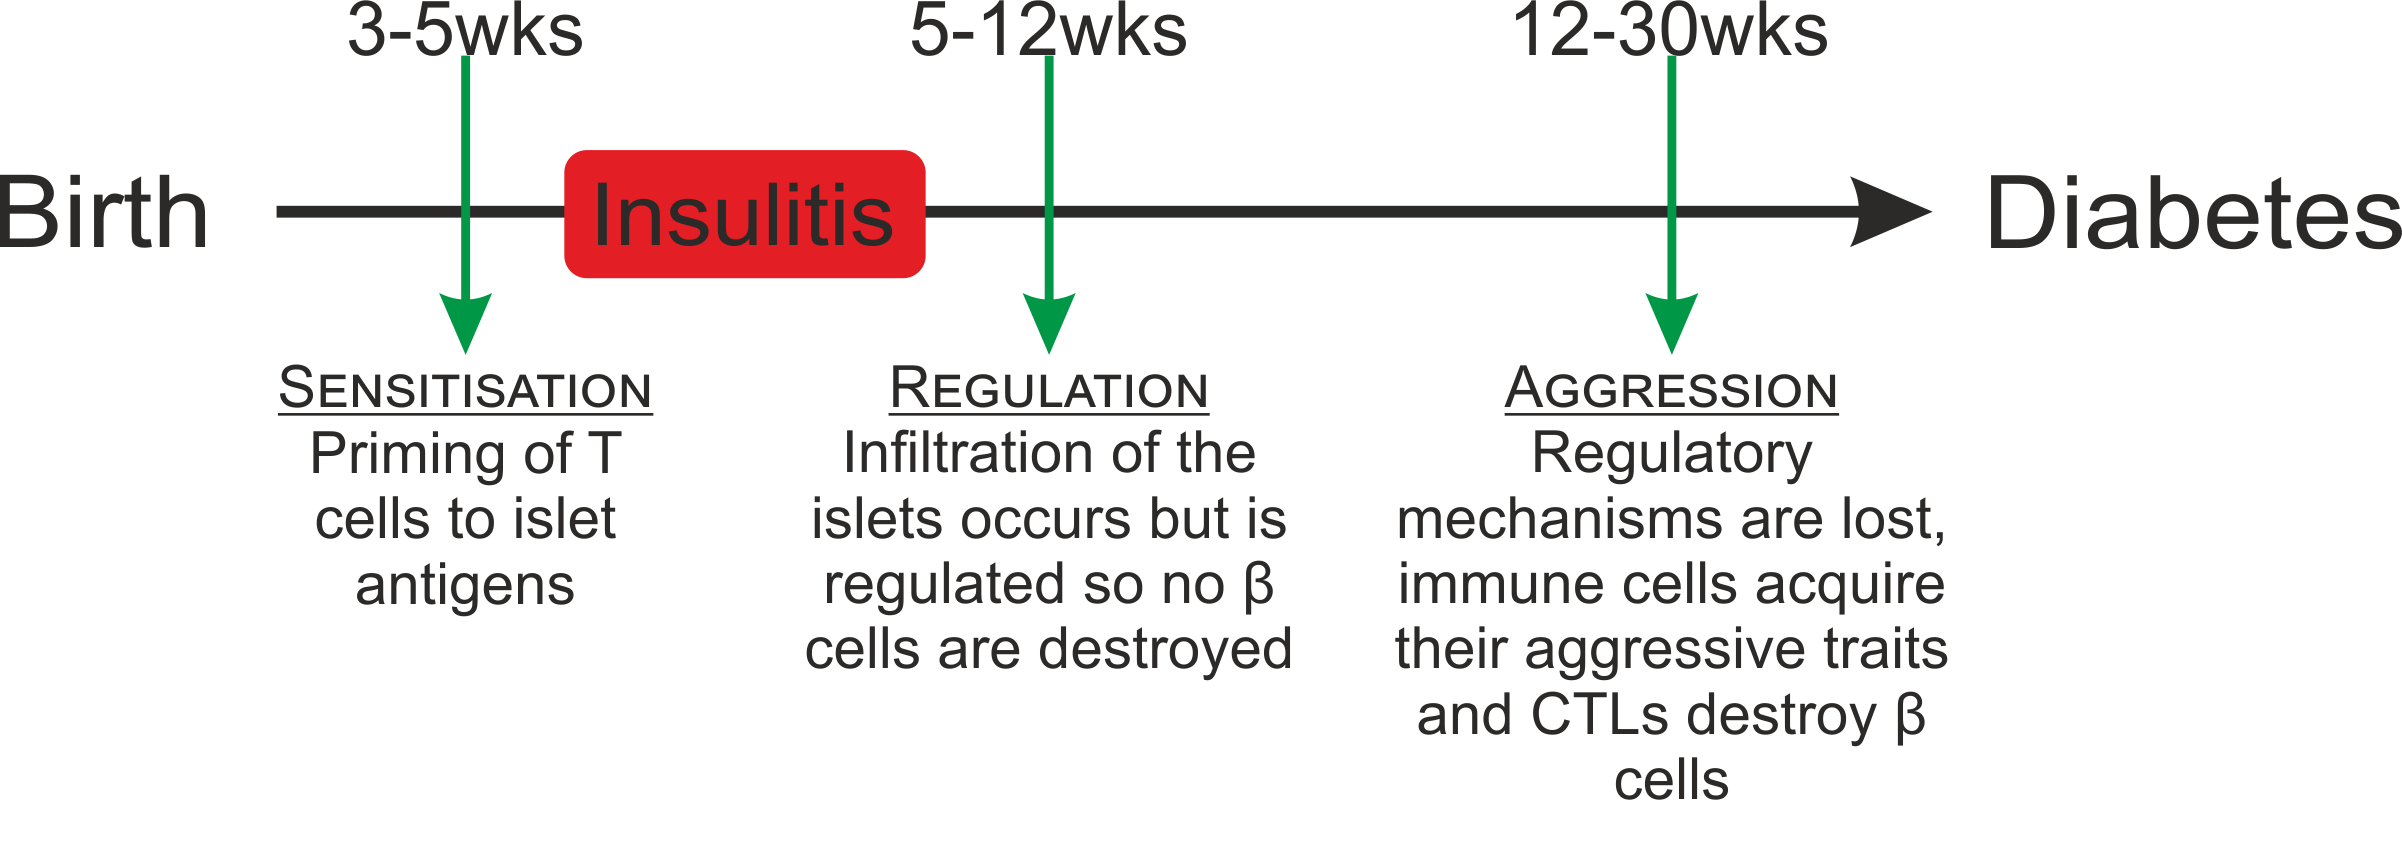
\includegraphics[width=\textwidth]{Figures/NODdisease.png}
\caption{Schematic representation of the T1D process in NOD mice}
\label{fig:diseasecourse}
\end{figure}

\begin{enumerate}
\item Sensitisation - Initial priming of T cells to islet antigen which takes place in the pancreatic lymph node (PLN)
\item Infiltration and insulitis - cells of the immune system move to the pancreatic islets and infiltrate the tissue. This is known as insulitis. For a while, the autoreactive cells' aggressive function is suppressed by regulatory mechanisms and no damage occurs
\item $\beta$ cell destruction - regulatory mechanisms become impaired and activated CD8\textsuperscript{+} T cells become cytotoxic T cells (CTLs) and begin to target and destroy $\beta$ cells. $\beta$ cells are believed to die by apoptosis \citep{Cnop2005}.
\end{enumerate}

It is believed that the NOD mouse is a relevant model for T1D research as it is thought the human disease follows a similar pathogenesis.
It has been seen in donated human diabetic tissues that there is infiltration of islets, albeit reduced compared to that seen in the NOD mouse \citep{Veld2014}, and it is thought that $\beta$ cell destruction is mediated by CTLs, similar to that seen in the NOD mouse \citep{Hanafusa2008}. 


Each of the stages of T1D development will be discussed further in the relevant sections below.


\subsection{Initiation of T1D}



It is not known what the initial trigger is in T1D that results in the release of islet antigen which normally remains hidden from the immune system.
However, genetic predisposition, such as T1D susceptible MHC, and environmental factors, such as infection \citep{Filippi2008} are thought to both be very important \citep{Knip2005}.
It is thought that both the innate and adaptive immune system have roles to play in initiation, through PRR binding, release of inflammatory cytokines and activation of T and B cells \citep{Diana2011}.

Autoantigens believed to be important in T1D are glutamic acid decarboxylase (GAD), insulin, islet-specific glucose-6-phosphatase catalytic subunit-related protein (IGRP) and insulinoma antigen-2 and 2$\beta$ (IA-2 and IA-2$\beta$) \citep{Green1999, Roep2012}.

%It is thought that the onset may be caused by DAMPs activating PRRs in the islets which results in the production of inflammatory cytokines and recruitment of immune cells to the islets \citep{Shin2015}.
%However, this does not provide an explanation as to why DAMPs are released in the first place.

%Viral infections have been thought to be implicated in the onset of T1D.
%The first of two potential mechanisms for this is molecular mimicry, where a viral antigen looks similar to an islet antigen and the T cell which can respond to the viral antigen is able to respond to the autoantigen as well.
%Evidence for this has been seen, such that GAD antigen is similar to a protein in Coxsackie B4 virus and in NOD mice with T1D susceptible MHC, they may be able to present both antigens to the same T cells \citep{Filippi2008}.
%However, it is more likely that bystander damage is mechanism by which viral infections are implicated in T1D onset.
%For this, a virus may infect $\beta$ cells and subsequent phagocytosis of the damaged $\beta$ cells releases antigens which can be presented to T cells and also causes release of proinflammatory cytokines \citep{Filippi2008}.
%This can result in T cell activation, recruitment of immune cells and a subsequent immune response.

%Another possibility involves the normal physiological process of pancreatic remodelling during growth and development. 
%Normally this occurs in a non-inflamed environment and as cells die and are replaced, the debris is cleared up by macrophages.
%The lack of inflammatory signals means that APCs do not become activated and therefore cannot present to T cells and mount an immune response \citep{Green1999}.
%However, if there is inflammatory signalling, or presence of inflammatory cytokines, the APCs are able to activate T cells and ellicit an immune response.
%This could suggest that the NOD mouse may be remodelling its pancreas in a more inflammatory environment, allowing the activation of APCs





\subsection{Infiltration and Insulitis}

Following sensistisation to islet antigen, immune cells then begin to move into the islets to form an infiltrate.
First only the edges of the islets are affected and this is known as peri-insulitis \citep{Thomas2000}.
Peri-insulitis is only seen in NOD mouse models and not human patients.
However, soon cells move into the islets too.
Infiltrating cells include, but are not restricted to, DCs, macrophages, B cells and T cells \citep{Brodie2008}.
It is believed that insulitis is the point at which tolerance to $\beta$ cell antigen is lost \citep{Thomas2000}.
There is evidence to suggest that this pathogenesis is not limited only to the NOD mouse as pancreatic samples from diabetic humans also reveal infiltrated islets.
Similar to the NOD mouse, this infiltrate contains CD8\textsuperscript{+} T cells, which have potential to become CTLs, other lymphocytes and APCs \citep{Hanafusa2008}.

\subsection{$\beta$ cell destruction}

Following non-destructive insulitis, immune cells gain their aggressive traits and beta cells begin to be destroyed.
The destruction of $\beta$ cells in NOD and human pancreatic islets is believed to be mediated by cytotoxic T lymphocytes (CTLs) \citep{Thomas2000, Brodie2008, Hanafusa2008}.
Only very few insulin-producing $\beta$ cells survive \citep{Oram2014, Veld2014}.



\section{B cell involvement in T1D}
\label{sec:BcellsinT1D}

It has been found that B cells have a critical role in diabetes pathogenesis and that without B cells, NOD mice are protected from the disease.
However, the role which these cells play in T1D pathogenesis is not known.
The main hypotheses relate to their two main physiological roles of antibody production and antigen presentation, along with cytokine secretion \citep{Hinman2014}.
However, there is also potential that they are interefering with the process of T cell negative selection which could also contribute to the disease process.

These potential roles will be discussed in more detail below.

\subsection{B cells are important in T1D}

Investigations into the role of B cells in T1D have revealed that the presence of B cells is crucial for T1D onset.

Evidence for this came in 1996 when \citet{Serreze1996} produced a mouse protected from diabetes by genetically depleting B cells from the NOD mouse.
These mice retained normal T cell populations and all known diabetes susceptibility genes, but lacked B cells suggesting that the diabetes protection resulted from the lack of B cells.
The resulting mouse was known as the NOD.Ig$\mu$\textsuperscript{null} mouse which had a functionally inactived Ig-$\mu$ chain and therefore cannot produce B cells.
Further evidence came in 1997 when \citet{Noorchashm1997} used anti Ig-$\mu$ antibody to deplete B cells from female NOD mice and compared the onset of insultis and blood glucose levels with control NOD mice which received whole rabbit IgG and therefore retained their B cell populations.
They found that insulitis and hyperglycaemia were not present in the Ig-$\mu$ treated mice, but were present in the controls.
Interestingly, they also found that following removal of Ig-$\mu$ antibody, the B cell pool repopulated and insulitis returned, giving further evidence that insulitis and diabetes are linked to B cell presence.

Further evidence for the importance of B cells in T1D pathogenesis has been shown more recently through the effectiveness of B cell depletion treatments in NOD mice in the prevention/delay of T1D onset.
It has been shown in both humans and mouse models that administration of anti-CD20 antibody during the early onset of T1D has an effect on slowing/preventing T1D progression.
In man, it was found that Rituximab (an anti-CD20 antibody) treatment in newly diagnosed type 1 diabetics preserved $\beta$ cell function for a year following treatment before the disease progressed again \citep{Pescovitz2009}.
In mouse models, it has been shown that anti-CD20 antibody treatment can prevent or slow T1D progression depending on the time point at which it is administered \citep{Xiu2008}.

As yet, there is no definitive answer as to the role of B cells in T1D.
However, it is thought that it relates either to their antigen-presenting or autoantibody producing functions, or both.

\subsection{Antibody production}

Autoantibodies are present in T1D and have in fact been useful in identifying candidate islet autoantigens \citep{Roep2012}.
However, the role that they play in the pathogenesis of T1D is not known.

To assess the potential role of autoantibodies, autoantibodies from diabetic NOD mice were transferred to NOD.Ig$\mu$\textsuperscript{null} mice to see if diabetes susceptibility could be transferred.
However, there was no change in diabetes protection so the mice remained disease free \citep{Serreze1998}.
This gives the impression that, while autoantibodies may be important in the disease, they are not sufficient to cause disease onset and are likely to not be the primary role of B cells in the T1D pathogenesis.

Further to this, the role of maternal autoantibodies in NOD offspring has been investigated.
\citet{Greeley2002} has shown that the removal of insulin autoantibodies from mothers of NOD offspring prevented T1D in offspring.
However, others, such as \citet{Koczwara2004nods} have shown that maternal autoantibodies have very little effect on the T1D progression in the offspring in NOD mice.
This shows that there is conflicting evidence for the role of autoantibodies in T1D.
The lack of clear cut evidence suggesting a vital role in T1D pathogenesis suggests that the production of autoantibodies is unlikely to be the only role of the B cell in T1D.

To assess the relative importance of autoantibody production versus antigen presentation by B cells in T1D pathogenesis, \citet{Wong2004} compared NOD.$\mu$MT mice (mice that are unable to rearrange their IgM heavy chain and therefore unable to progress beyond the pro B cell stage \citep{Kitamura1991}) with transgenic mice that were unable to secrete antibodies but still displayed a normal BcR.
They found that the transgenic mice had an increased incidence of T1D compared to the NOD.$\mu$MT controls, suggesting that B cells drive T1D pathogenesis via an antibody independent mechanism \citep{Wong2004}.



\subsection{Antigen presentation}


Following the finding that autoantibodies are likely to not be the principle mechanism of action for B cells in T1D pathogenesis, \citet{Serreze1998} also looked into the antigen presenting capacity of B cells.
In particular, their ability to present GAD and ellicit T cell responses was investigated.
It was noted that B cells were critical for the initial priming of T cells to GAD, shown by the lack of spontaneous T cell response to it in NOD.Ig$\mu$\textsuperscript{null} mice compared to control NODs.
However, it seemed that following initial priming, other APCs were sufficient to present to T cells on restimulation with GAD antigen.
This could explain why transfer of T cells from NOD mice into other mice lacking B cells such as NOD/SCID mice (which have no T or B cells and are protected from T1D) can cause disease as APCs other than B cells in the recipient mice would be sufficient to reactivate the transferred T cells \citep{Charlton2001}.

B cells acting as APCs to activate autoreactive T cells was further investigated by determining the effect of rendering B cells deficient of MHC Class II.
In this study, I-A\textsuperscript{
g7} (The MHC Class II expressed in NOD mice \citep{Stratmann2000}) expression was deficient in B cells but normal on other non-B cell APCs \citep{Noorchashm1999}.
These mice were resistent to T1D, despite the presence of normal APCs. 
This suggests that it is a process relating to MHC Class II and therefore, antigen presentation, that B cells are required for.


B cell specificity to self antigen is important in T1D pathogenesis.
Evidence for this comes from the finding that T1D onset can be accelerated by modifying the BcR to be more reactive to insulin.
In this study, B cells were manipulated so that 1-3\% of the B cell population were insulin specific.
Controls were also modified using similar transgenes but these gave limited insulin binding capabilities.
It was seen that the mice with insulin specific B cells developed T1D at a much faster rate than controls, suggesting that antigen specifity of B cells is an important determinant of T1D onset \citep{Hulbert2001}.

Further evidence for the antigen presentation capacity of B cells is that NOD B cells that have infiltrated the islets in T1D appear to have increased levels of costimulatory molecules, B7-1 and B7-2 \citep{Hussain2005}. 
This could suggest that they have an increased ability to present to, and activate, T cells which could aid the progression of the diabetic process in the islets.

In terms of activating T cells, it is thought that CD8\textsuperscript{+} T cells are the main culprits for $\beta$ cell destruction in T1D.
As mentioned in \cref{subsec:Tcellactivation}, to activate CD8\textsuperscript{+} T cells, APCs have to present their cognate antigen on MHC Class I via the process of cross-presentation.
Whilst this process is usually carried out by DCs, there is evidence that B cells can cross present islet antigen to CD8\textsuperscript{+} T cells in the PLN.
This was shown by a decrease in activated CD8\textsuperscript{+} T cell population both in B cell deficient mice and in mice whose B cells have been rendered MHC Class I deficient \citep{Marino2012}.
This gives the impression that B cells could be playing an important role in activating CD8\textsuperscript{+} in the diabetics process, allowing them to become CTLs which could destroy $\beta$ cells.

The evidence to date suggests that presentation of self antigens to autoreactive T cells are the principle action of B cells in the pathogenesis of T1D.



%Resting B cells are unable to prime T cells.
%The reason for this is that they do not express any costimulatory moecules and therefore are unable to deliver signal 2 for T cell activation.
%However, once B cells are activated by T cells, they become activated and are then able to act as antigen presenting cells.
%B cells are efficient antigen presenting cells as they can process whole proteins and express multiple different epitopes from the same protein, thus activating a bigger population of T cells. 

%Cross presentation of antigen to present to T cells?


\section{Thymic B cells}
\label{sec:thymicBcells}
 
It is normal for B cells to be present in the thymus in small numbers \citep{Isaacson1987, Akashi2000, Miyama1988} of non diabetic humans \citep{Isaacson1987} and mice \citep{Akashi2000}. 
However, in the NOD mouse, this population of B cells is dramatically increased \citep{OReilly1994, Serreze1998}.
It is not known how B cells come to populate the thymus, it is thought to either be as a result of migration to the thymus or development from progenitors within the thymus.
Development is more likely due to the fact that some thymic progenitors do have B cell potential \citep{Porritt2004} and developing pro and pre B cells are seen in the thymus \citep{Akashi2000}.

%\begin{figure}
%\includegraphics{Figures/MigrationvsDevelopment.png}
%\caption{Normal B cell development occurs in the bone marrow and normal T cell development occurs in the thymus.
%However, it may be that B cell progenitors are moving to the thymus to develop into B cells within the thymus}
%\label{fig:migrationvdevelopment}
%\end{figure}

%This increase in thymic B cells has previously been confirmed by flow cytometry carried out in our lab to compare B cells in the bone marrow and thymus of NOD mice and control, non diabetic B6 mice.
%As shown in \cref{fig:JVgraph}, the presence of B cells in the NOD mouse thymi is significantly increased compared to B6 thymi and the difference between the strains increases as the mice age. (Acknowldegements to Jennifer Varian for the graph).

%\begin{figure}
%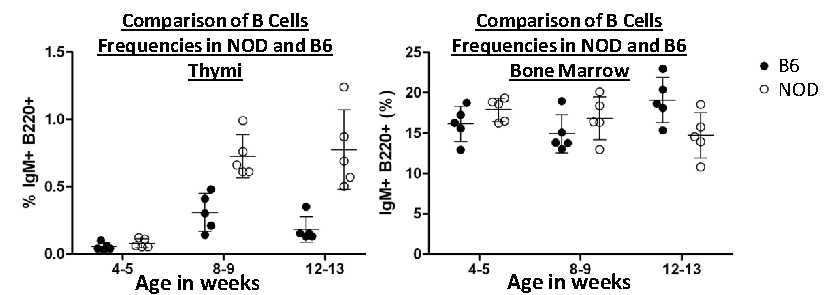
\includegraphics[width=\textwidth]{Figures/JVgraph.pdf}
%\caption{B cells increase in the NOD thymus but not bone marrow compared to B6 controls.
%The increase is more pronounced as mice age}
%\label{fig:JVgraph}
%\end{figure}

The increase in B cells is intriguing as it appears to be age-related and correlates with the progression of the disease in the NOD mouse.
This could suggest that either thymic B cells are involved in driving the disease progression, or it may be that they are a result of disease progression.

This increase in thymic B cells is not entirely unique to T1D in NOD mice, it is also a phenomenon seen in other autoimmune diseases such as myasthenia gravis \citep{Vrolix2014, Christensson1988} and therefore unravelling the origin and function of thymic B cells in the NOD mouse, may have benefits beyond those in the field of T1D.

The function of thymic B cells is not known.
However, it is thought they may have a role in contributing to T cell negative selection due to the fact they are seen to position themselves next to mTECs in the thymus \toref{Starr2003, Perera2013}.



\section{Project Aims}

\cref{fig:summarydiagram} outlines the current understanding of B cell development in the bone marrow, T cell development in the thymus and potential intrathymic B cell development.

This project aims to understand more fully the potential pathway of intrathymic B cell development.
These are the main questions that this project aims to investigate:
\begin{itemize}
\item Are early B cell progenitors and developing B cells present in the thymus of NOD mice?
\item Is the thymus able to support B cell receptor rearrangement on developing thymic B cells?
\item Does the thymus of the NOD mouse look different to NOD.$\mu$MT B cell KO mice in terms of B cell progenitors/developing B cells?
\item How does the NOD thymus compare to the nondiabetic B6 thymus in terms of intrathymic B cell development?
\end{itemize}

\begin{figure}
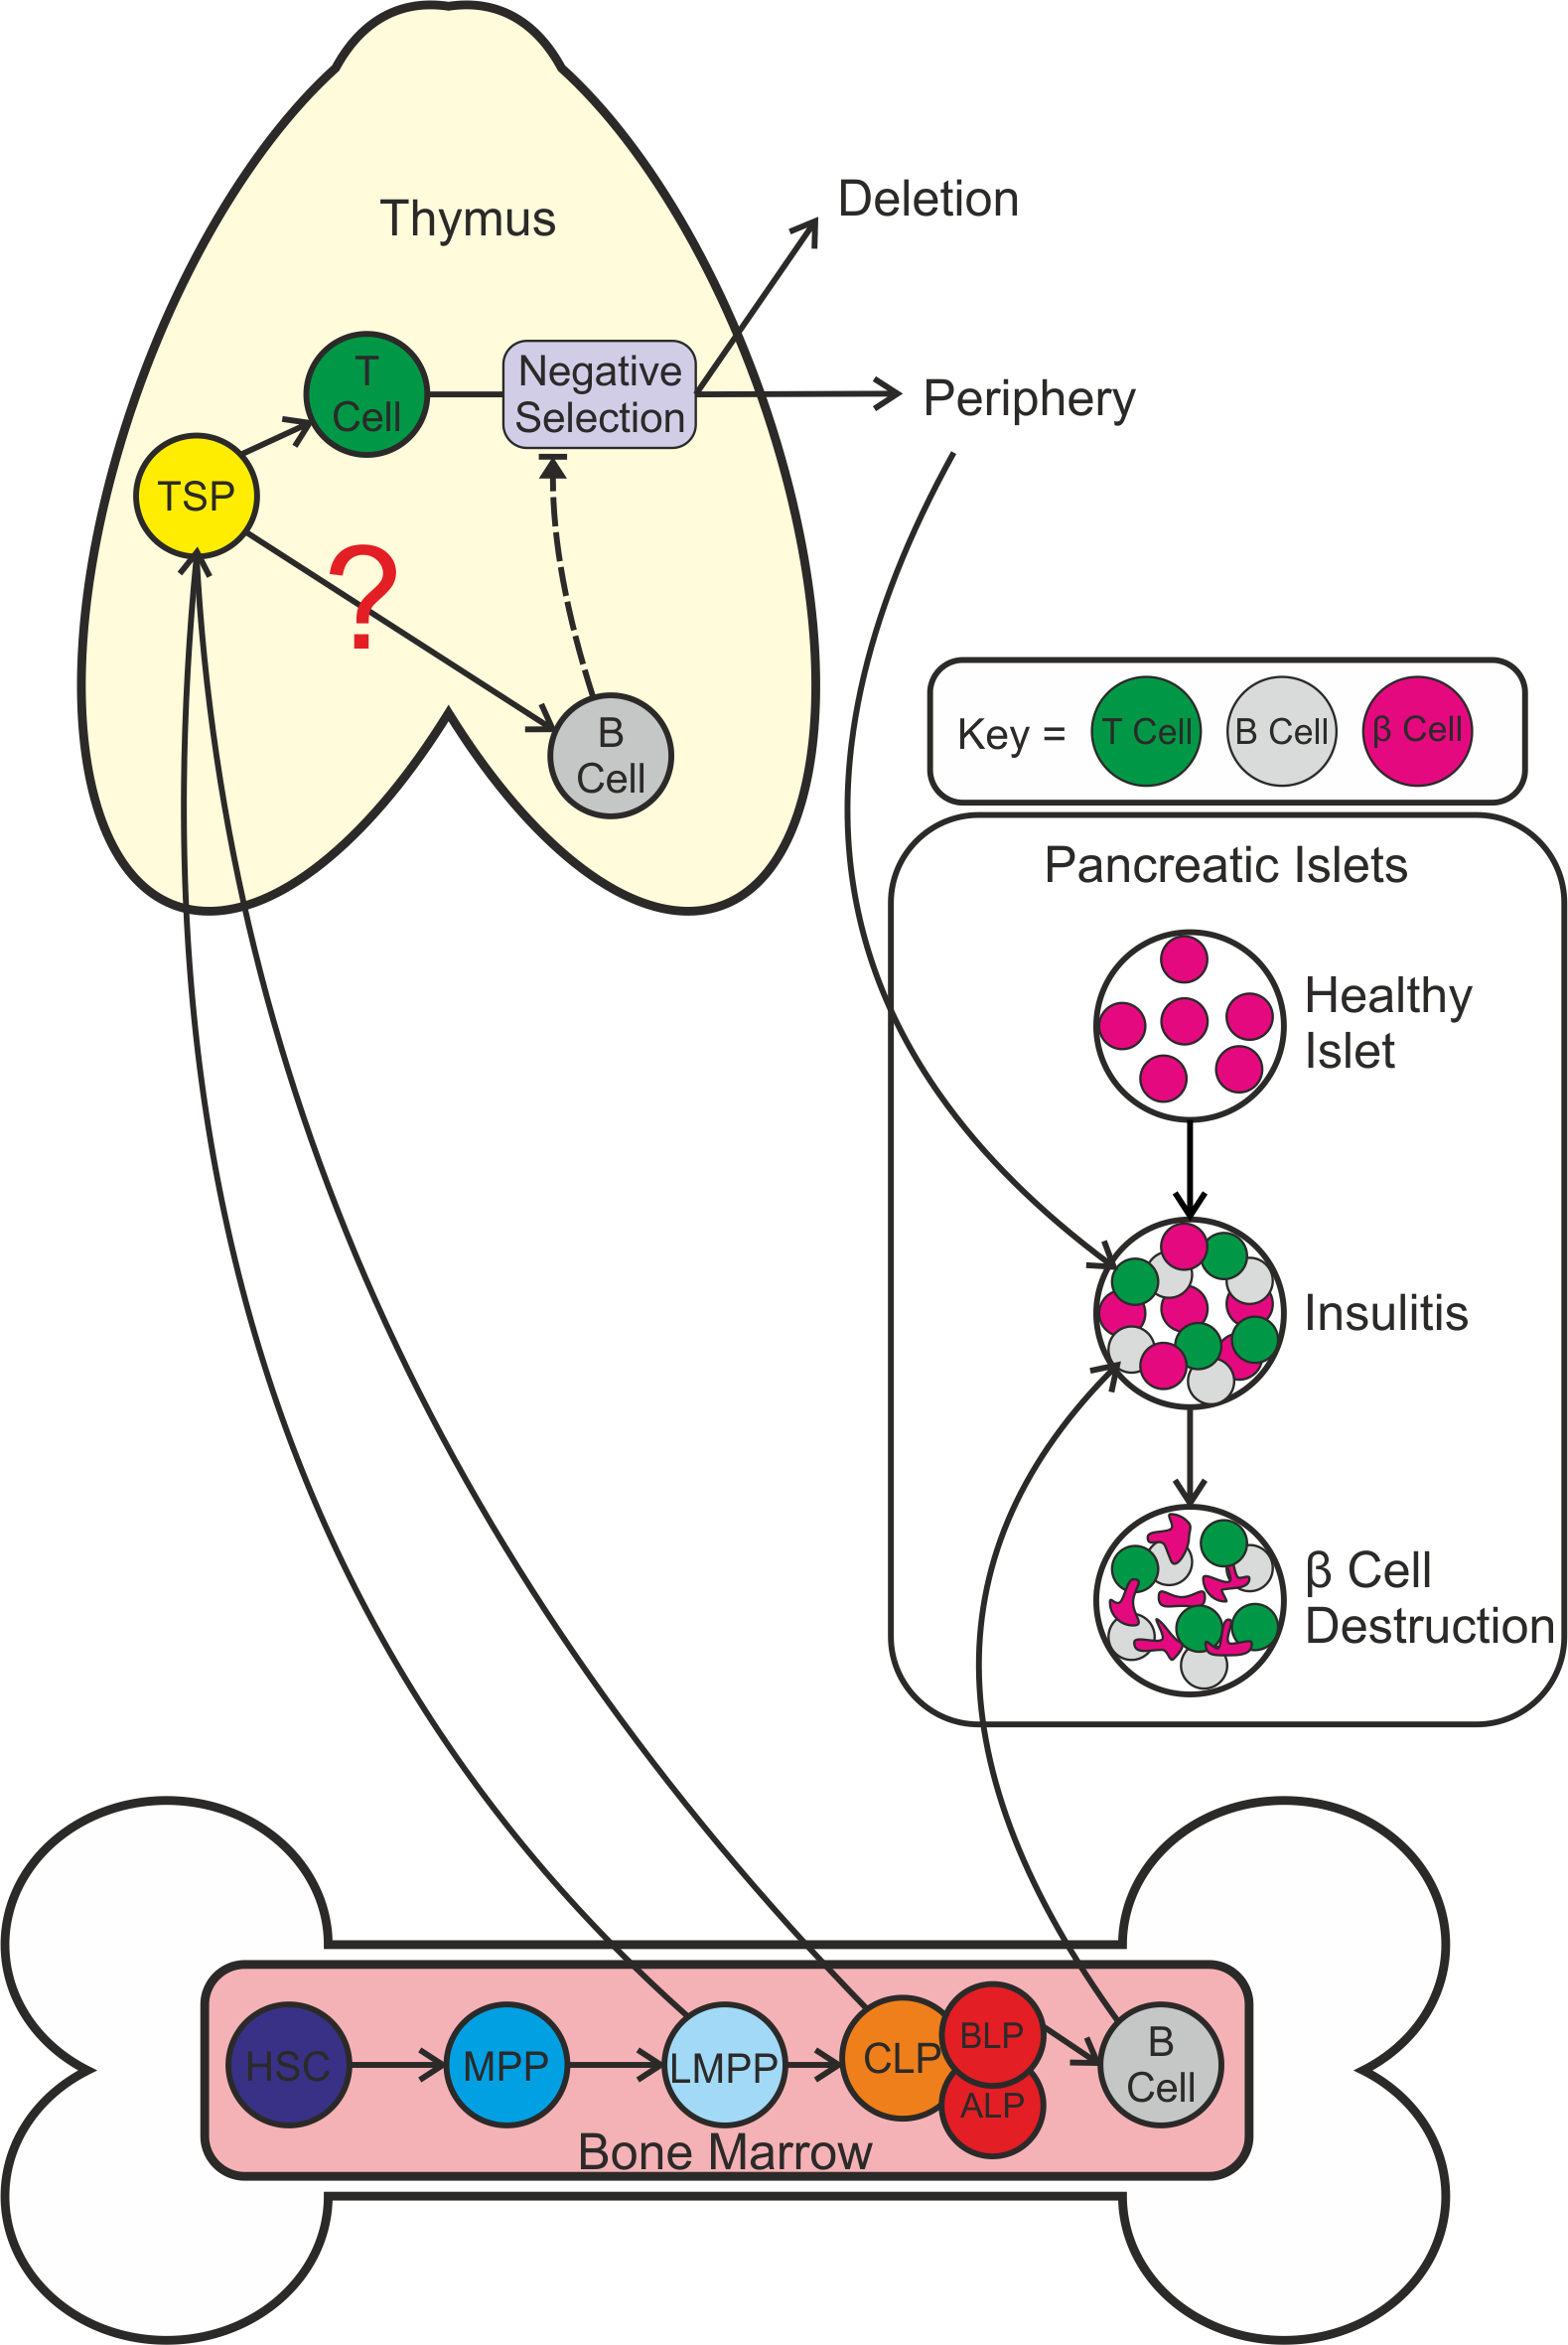
\includegraphics[width=\textwidth]{Figures/Introductorydiagram.png}
\caption[Diagrammatical overview of project]{B cells develop in bone marrow, T cells develop in thymus. 
In seeding of the thymus with TSPs destined for the T cell fate, it may be that some progenitors are retaining B cell potential.
These cells may be differentiating into B cells in the thymus, resulting in a population of thymic B cells.
T cells go through negative selection in the thymus as the first stage of tolerisation. 
Those which survive this process are released in the periphery.
In the case of T1D, healthy islets become infiltrated with immune cells including T and B cells (potentially including some of thymic origin) and subsequently, insulin-producing $\beta$ cells are destroyed by CTLs.
It may be that thymic B cells are contributing to T cell negative selection in some way (black dashed arrow).}
\label{fig:summarydiagram}
\end{figure}




































